% /Users/pikachu/books/payments-book/src/parts/part5/ch26-payment-gateway.tex
\chapter{Платёжный шлюз изнутри}
\label{ch:gateway}
\margintoc


\begin{kaobox}[title=Что вы узнаете из этой главы]
  Как платёжный шлюз раскладывает один запрос мерчанта на несколько
  внутренних шагов; чем интеллектуальная маршрутизация отличается
  от каскадной и почему их опасно смешивать; как интеграционная
  модель задаёт PCI scope мерчанта; почему timeout нельзя
  автоматически считать отказом; и как JSON-запрос превращается в сообщение
  \iso{8583}, не делая сам шлюз системой учёта денег.
\end{kaobox}

Один запрос мерчанта: \codeword{POST} к \endpoint{/v1/payments}
на оплату заказа. Снаружи это обычный JSON поверх HTTPS. Внутри
же один и тот же запрос проходит через последовательность решений,
и ошибка в любом звене меняет либо риск, либо конверсию, либо
PCI scope. Чтобы понять, где здесь заканчивается интеграция
и начинается архитектура, разберём этот путь по шагам.

\section{Анатомия шлюза}
\label{sec:gw-anatomy}

В предыдущих частях книги мы двигались вдоль жизненного цикла
транзакции, рассматривая её с точки зрения протоколов, платёжных
систем и операционных процессов. Теперь вопрос звучит иначе:
что именно должно произойти внутри системы, чтобы один запрос
мерчанта превратился в корректную, наблюдаемую и управляемую
авторизацию. Ответ на этот вопрос и даёт платёжный шлюз
(payment gateway).

\begin{kaobox}[title={Определение: Платёжный шлюз, процессор, оркестратор}, colback=blue!4, colbacktitle=blue!15]
  Три термина часто используют как взаимозаменяемые, но на деле
  они описывают разные уровни абстракции. \textbf{Платёжный шлюз}
  (payment gateway) принимает платёжные запросы от мерчанта
  по высокоуровневому API и переводит их в протоколы карточных
  сетей и банков-эквайеров. \textbf{Платёжный процессор}
  (payment processor) непосредственно обрабатывает авторизацию,
  клиринг и settlement и часто имеет прямое подключение
  к карточным сетям. \textbf{Платёжный оркестратор}
  (payment orchestrator) маршрутизирует транзакции между
  несколькими шлюзами или процессорами по заданным правилам.
  Границы между ролями часто размыты: крупные провайдеры
  платёжных услуг (PSP) вроде Stripe или Adyen совмещают
  все три уровня в одном продукте.
\end{kaobox}

Независимо от названия конкретного продукта, внутри платёжного
шлюза почти всегда можно выделить пять ключевых компонентов,
через которые проходит каждая транзакция: слой приёма API-запросов,
модуль оценки риска, модуль маршрутизации, хранилище токенов
и модуль авторизации, отправляющий запрос банку-эквайеру
или напрямую карточной сети.

Порядок, в котором эти компоненты вызываются, не случаен. Он
определяет и архитектурные свойства системы, и её PCI scope.
Рассмотрим типичный путь запроса.

Мерчант отправляет HTTPS-запрос на API шлюза — например,
\codeword{POST} к \endpoint{/v1/payments} с JSON-телом, содержащим
сумму, валюту, данные карты или токен и метаданные заказа.
Слой приёма API-запросов валидирует сообщение, проверяет
аутентификацию (API key или OAuth token), обеспечивает
идемпотентность (об этом подробнее в разделе \ref{sec:gw-reliability})
и передаёт нормализованное внутреннее представление транзакции
следующему компоненту — модулю оценки риска.

Модуль оценки риска применяет к транзакции набор правил и моделей:
проверки частоты повторов (velocity checks), сопоставление
геолокации, отпечаток устройства, а в более зрелых системах ---
скоринговую модель, оценивающую вероятность мошенничества.
Результатом становится одно из трёх решений: пропустить
транзакцию дальше, отправить её на дополнительную проверку
по 3-D Secure или отклонить. Подробно устройство антифрод-систем
разобрано в главе \ref{ch:fraud}; здесь важен сам порядок:
проверка риска работает \emph{до} авторизации, потому что
подозрительную транзакцию дешевле остановить заранее, чем потом
разбирать chargeback.

Если модуль оценки риска пропустил транзакцию, она попадает в модуль маршрутизации,
который определяет, через какого эквайера (или какой процессор)
отправить авторизационный запрос. Логика маршрутизации —
одна из самых коммерчески значимых частей шлюза, и мы посвятим
ей отдельный раздел (\ref{sec:gw-routing}).

На следующем шаге, если мерчант передал полный PAN, шлюз заменяет
его токеном из хранилища токенов: PAN сохраняется в зашифрованном
хранилище, а дальше по внутреннему конвейеру и в ответе мерчанту
циркулирует только токен. Это сужает CDE (cardholder data environment)
до одного компонента и радикально сокращает PCI scope всей
системы — механизм, подробно описанный в главе
\ref{ch:pci-dss}. Если же мерчант с самого начала прислал
сетевой токен (DPAN), хранилище может не участвовать, но шлюз
всё равно проверяет ограничения домена токена (token domain
restriction) и при необходимости запрашивает у TSP актуальную
криптограмму (см. главу \ref{ch:tokenization}).

Наконец, модуль авторизации формирует сообщение \iso{8583}
(или его эквивалент в API-протоколах новых эквайеров),
отправляет запрос по защищённому каналу банку-эквайеру,
получает ответ, преобразует код ответа в формат API шлюза
и возвращает результат мерчанту. Весь путь — от HTTPS-запроса
до ответа — укладывается в одну-две секунды; основная часть
времени уходит на ожидание ответа эмитента через карточную сеть.

\begin{marginfigure}
  \centering
  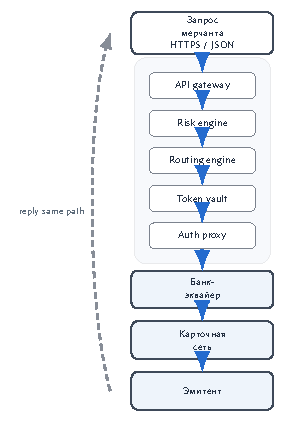
\includegraphics[width=\linewidth]{assets/figures/ch26-payment-gateway/gateway-components.pdf}
  \caption{Компоненты платёжного шлюза.}
  \label{fig:gateway-components}
\end{marginfigure}

Уже на этом минимальном маршруте видно главное свойство шлюза:
каждый следующий компонент получает более узкое и лучше
определённое представление транзакции, чем предыдущий. Именно
из этого вырастают и требования к изоляции данных, и PCI scope,
и ограничения на отказные режимы.

\section{Интеллектуальная маршрутизация}
\label{sec:gw-routing}

Как только у шлюза появляется больше одного эквайера, задача
меняется. Теперь мало просто доставить авторизационный запрос:
нужно ещё и решить, куда его отправить, чтобы не проиграть
одновременно в стоимости, доле одобрений и времени ответа.
Именно в этот момент шлюз перестаёт быть простым прокси
и превращается в модуль маршрутизации.

\subsection*{Три оси оптимизации}

Первая ось — \textbf{стоимость}. Разные эквайеры предлагают
разные тарифы, а interchange fee зависит от типа карты,
MCC мерчанта, региона эмитента и десятков других параметров.
Модуль маршрутизации может выбрать эквайера с минимальной
стоимостью для конкретной комбинации условий — например,
направить внутрироссийскую транзакцию по карте Мир через
эквайера с более выгодным тарифом НСПК, а трансграничную
транзакцию --- через другого, у которого ниже валютная
наценка.

Вторая ось — \textbf{доля одобрений}. Разные эквайеры
показывают разную долю одобрений для одних и тех же BIN-диапазонов.
Причины могут быть техническими, коммерческими или регуляторными:
качество подключения к сети, скорость ответа, репутация мерчанта
у конкретного эквайера, локальный или трансграничный маршрут.
Накапливая статистику по BIN, стране и сумме, модуль маршрутизации
может направить транзакцию туда, где вероятность одобрения выше.
Разница между удачным и неудачным маршрутом достигает 3--5
процентных пунктов, что для крупного мерчанта превращается
в миллионы рублей выручки.

Третья ось — \textbf{латентность}. Для мерчанта, работающего
в реальном времени, важно, чтобы ответ пришёл быстро: если
один эквайер стабильно отвечает за 300~мс, а другой --- за
1200~мс, модуль маршрутизации при прочих равных предпочтёт
первый, потому что каждая лишняя секунда в сценарии оплаты
снижает конверсию.

Эти три оси неизбежно конфликтуют: самый дешёвый эквайер
может иметь худшую долю одобрений, а самый быстрый оказаться
самым дорогим. Задача модуля маршрутизации --- найти рабочий
оптимум в рамках ограничений, заданных мерчантом: \enquote{минимизировать
стоимость при доле одобрений не ниже X\% и p95 латентности
не более Y~мс}. Продвинутые системы решают такую задачу
как адаптивное распределение трафика; в литературе этот подход
часто описывают моделью multi-armed bandit.

\subsection*{Каскадная маршрутизация}

Каскадную маршрутизацию часто путают с интеллектуальной, хотя
она решает другой вопрос. Если первый эквайер вернул мягкий
отказ (soft decline, например \rc{05} --- Do Not Honor), шлюз
автоматически повторяет транзакцию через второго эквайера.
Логика проста: мягкий отказ одного маршрута ещё не означает,
что транзакция в принципе невозможна. Другой эквайер может
получить иной ответ от того же эмитента, особенно если его
авторизационный запрос отличается: другой BIN эквайера, другой
MCC, другое значение Terminal ID.

\begin{kaobox}[title=Важно, colback=red!5, colbacktitle=red!20]
  Каскадная маршрутизация — \emph{не} то же самое, что обычный
  повтор. Она отправляет транзакцию \emph{другому} эквайеру
  после мягкого отказа от первого; повтор же идёт \emph{тому же}
  эквайеру, обычно спустя некоторое время. Путаница между
  этими сценариями и приводит к дублям: если шлюз повторил
  запрос тому же эквайеру, а первый ответ лишь задержался,
  эмитент увидит два авторизационных запроса и может одобрить
  оба. Каскад сам по себе не создаёт дубля на стороне первого
  эквайера, но создаёт другой риск: задержавшийся ответ от
  первого маршрута может прийти уже после того, как второй
  успел получить одобрение. Поэтому грамотная реализация должна
  уметь немедленно отправлять reversal первой авторизации,
  если она материализовалась с опозданием.
\end{kaobox}

Каскадная маршрутизация полезна для мягких отказов, но
бесполезна и даже вредна для жёстких отказов (hard decline),
таких как \rc{14} --- Invalid Card Number или \rc{54} ---
Expired Card. Повторная попытка здесь заведомо не изменит
исход, а лишние авторизационные запросы нарушают правила
платёжных систем по повторам: \scheme{Visa} и \scheme{Mastercard}
ограничивают их количество и штрафуют за превышение
(см. главу \ref{ch:decline-management}). Поэтому модуль
маршрутизации должен различать эти два класса отказов
по коду ответа и включать каскад только в первом случае.

Итак, интеллектуальная маршрутизация отвечает на вопрос,
\enquote{куда лучше вести первую попытку}, а каскадная ---
на вопрос, \enquote{что делать после мягкого отказа}. Смешивать
эти две логики опасно именно потому, что у них разные цели
и разные отказные режимы.

\section{Интеграционные модели}
\label{sec:gw-integration}

Способ подключения мерчанта к платёжному шлюзу определяет
не только внешний вид сценария оплаты, но и то, где проходит
граница ответственности за карточные данные. Иначе говоря,
это одновременно решение о пользовательском опыте, архитектуре
и PCI scope мерчанта.

\begin{kaobox}[title={Определение: Hosted payment page}, colback=blue!4, colbacktitle=blue!15]
  Hosted payment page (HPP) — веб-страница, размещённая
  на серверах платёжного шлюза, на которую мерчант перенаправляет
  покупателя для ввода данных карты. Мерчант не видит,
  не принимает и не передаёт карточные данные — они вводятся
  и обрабатываются целиком на стороне шлюза.
\end{kaobox}

\subsection*{Hosted payment page (перенаправление)}

В модели HPP мерчант инициирует платёжную сессию через API шлюза
и получает URL, на который перенаправляет покупателя. Покупатель
вводит данные карты на странице шлюза, шлюз обрабатывает транзакцию
и возвращает покупателя на сайт мерчанта с результатом. Параллельно
шлюз отправляет мерчанту асинхронное уведомление с финальным
статусом.

Главное преимущество HPP — минимальный PCI scope: поскольку
карточные данные никогда не проходят через серверы мерчанта,
он может заполнить SAQ A — самый короткий опросник самооценки
PCI DSS, содержащий порядка 30 контролей вместо 300+
в SAQ D (см. главу \ref{ch:pci-dss}). Для небольших мерчантов,
у которых нет выделенной команды безопасности, это часто
единственный реалистичный вариант.

Недостаток --- потеря контроля над пользовательским сценарием:
перенаправление прерывает поток оплаты, страница шлюза может
выбиваться из визуального языка сайта, а обратный переход
после оплаты не всегда проходит гладко. Кроме того, лишний
шаг в воронке может снижать конверсию на 1--3\%, что для
крупной онлайн-торговли уже ощутимо.

\subsection*{Встроенная форма (iFrame / JavaScript SDK)}

Компромиссная модель выглядит так: мерчант встраивает
в свою страницу платёжную форму, предоставляемую шлюзом
в виде iFrame или готового JavaScript-компонента.
Визуально форма
выглядит как часть сайта мерчанта, но технически данные карты
вводятся внутри iframe, контролируемого шлюзом, и отправляются
напрямую на серверы шлюза, минуя серверы мерчанта.

Эта модель сохраняет больше контроля над интерфейсом: мерчант
может стилизовать форму, не разрывать сценарий оплаты и при
этом претендовать на SAQ A или SAQ A-EP. Разница зависит
от деталей реализации и от того, проходят ли карточные данные
через JavaScript мерчанта хотя бы транзитом.

\begin{kaobox}[title=На практике]
  PCI DSS v4.0.1 ввёл требование 6.4.3, обязывающее контролировать
  все JavaScript-скрипты, загружаемые на платёжной странице.
  Даже если карточные данные вводятся в iFrame шлюза, вредоносный
  скрипт на странице мерчанта может перехватить ввод через
  подложный слой или keylogger ещё до того, как данные попадут
  в iFrame. Поэтому
  SAQ A при использовании iFrame теперь требует от мерчанта
  инвентаризации и мониторинга клиентских скриптов —
  контроль, которого раньше не было.
\end{kaobox}

\subsection*{Прямая интеграция через API (server-to-server)}

В этой модели мерчант собирает данные карты на своей стороне
(через собственную форму) и отправляет их на API шлюза
в серверном запросе. Мерчант получает полный контроль над
интерфейсом и может реализовать произвольную предварительную
логику: проверку адреса, предавторизацию, разделение платежа
между несколькими получателями. Но платит за это
максимальным PCI scope: карточные данные проходят через его серверы,
что требует SAQ D или полного ROC (Report on Compliance) —
сотни контролей, ежегодный аудит QSA и квартальные ASV-сканы.

Этот путь выбирают крупные мерчанты и платёжные платформы,
которые уже имеют PCI DSS Level 1 сертификацию и для которых
прямой контроль над данными — конкурентное преимущество
(например, возможность реализовать собственное защищённое
хранилище токенов или оптимизировать логику повторов
на уровне PAN).

\begin{kaobox}[title=На практике]
  Выбор интеграционной модели --- ещё и бизнес-решение. Разумно
  начинать с iFrame или SDK: это даёт приемлемый пользовательский
  опыт при минимальном PCI scope. Переходить на server-to-server
  стоит только тогда, когда ограничения встроенной формы начинают
  блокировать конкретный сценарий --- например, если нужно
  реализовать Card-on-File с прозрачной для покупателя токенизацией
  или каскадную маршрутизацию на уровне PAN.
\end{kaobox}

Во всех трёх моделях меняется не только форма интеграции,
но и глубина участия мерчанта в зоне карточных данных. Поэтому
разговор об этих трёх моделях всегда
оказывается одновременно разговором и о продукте, и о контролях.

\section{Надёжность и наблюдаемость}
\label{sec:gw-reliability}

Ценность шлюза проверяется не тогда, когда всё идёт по плану,
а тогда, когда ответ запаздывает, внешний вызов теряется,
а мерчант нажимает \enquote{повторить}. Надёжный шлюз отличается
от хрупкого прежде всего дисциплиной обращения с неопределённостью.

\subsection*{Идемпотентность}

Идемпотентность — свойство операции, при котором повторный вызов
с тем же набором параметров даёт тот же результат, что и первый,
без побочных эффектов. В контексте платежей это выглядит так:
если мерчант отправил запрос на авторизацию, не получил ответа
(timeout, сетевой сбой) и повторил его с тем же idempotency key,
шлюз должен вернуть результат первой попытки, а не создавать
вторую транзакцию.

Для этого шлюз хранит устойчивое сопоставление между
\codeword{idempotency_key} и \codeword{transaction_id}
в хранилище с гарантированной консистентностью, обычно
в реляционной базе данных с уникальным индексом по ключу.
Время жизни idempotency key, как правило, составляет от
24~часов до 7~дней: слишком короткий срок не защитит
от задержанных повторов, слишком длинный бессмысленно
раздувает хранилище.

\begin{kaobox}[title=Важно, colback=red!5, colbacktitle=red!20]
  Идемпотентность на уровне шлюза не заменяет идемпотентность
  на уровне эквайера. Если шлюз отправил авторизацию эквайеру,
  не получил ответа и отправил повторно — эквайер может
  обработать оба запроса. Шлюз должен либо использовать
  \de{11} (STAN) + \de{37} (RRN) для дедупликации
  на стороне эквайера, либо реализовать сценарий
  \enquote{authorize-then-check}: при timeout отправлять не повтор,
  а запрос статуса (status inquiry, \mti{0120} или проприетарный запрос),
  и только если статус — \enquote{не найдено} — повторять
  авторизацию.
\end{kaobox}

\subsection*{Обработка timeout}

Timeout --- одна из самых неприятных ситуаций в платёжном
процессинге, потому что отсутствие ответа --- это \emph{не}
отказ. Если шлюз отправил авторизационный запрос эквайеру
и не получил ответа в течение установленного порога, обычно
30--60~секунд, возможны как минимум три исхода: запрос вообще
не дошёл; запрос дошёл, эмитент одобрил транзакцию, но ответ
потерялся на обратном пути; запрос дошёл, эмитент отказал,
и этот ответ тоже потерялся. В момент timeout шлюз не может
различить эти три случая, и именно это делает ситуацию опасной.

Наихудший из трёх исходов — (б): деньги заблокированы на карте
держателя, эмитент считает транзакцию одобренной, а мерчант
не знает об этом и может попытаться повторить платёж, создав
двойное списание. Правильная стратегия — после timeout
отправить reversal (\mti{0420}) по тому же STAN и RRN:
если оригинальная авторизация прошла, reversal её отменит;
если не прошла — reversal будет отклонён как not found,
что тоже информативно. Только после reversal шлюз может
безопасно вернуть мерчанту статус \enquote{неуспешно}
или предложить повторить попытку.

\subsection*{Дедупликация}

Идемпотентность решает лишь часть проблемы. Дедупликация
как защита от двойной обработки одной и той же транзакции
работает на нескольких уровнях. На уровне API она опирается
на idempotency key. На уровне внутреннего конвейера --- на
уникальность комбинации STAN + RRN + amount + timestamp,
которая позволяет отлавливать дубли, проскочившие мимо
идемпотентности, например при каскадной маршрутизации, когда
два эквайера получают запрос с разными STAN, но за одну и ту
же покупку. На уровне денежных состояний дедупликацию берёт
на себя внутренний реестр обязательств из главы
\ref{ch:internal-ledger}, а на уровне внешних файлов и банковской
выписки --- сверка из главы \ref{ch:reconciliation}.

\subsection*{Webhooks и гарантия доставки}

Платёжный поток редко заканчивается в момент синхронного
API-ответа. Результат транзакции возвращается мерчанту
двумя путями: синхронно --- в ответе на запрос --- и асинхронно
--- через обратный HTTP-вызов (webhook) на указанный URL.
Webhook нужен не только потому, что синхронный ответ может
не дойти, но и потому, что после первого ответа появляются
новые внешние события: завершился 3-D Secure challenge,
пришёл capture, сработал refund или поступило позднее
обновление статуса от процессора.

Гарантия доставки webhook строится по принципу \enquote{как
минимум один раз} (at-least-once):
шлюз отправляет POST-запрос на URL мерчанта и ожидает ответ
с HTTP-кодом 2xx; если ответ не получен, шлюз повторяет попытку
с экспоненциальной задержкой --- обычно через 5~секунд,
30~секунд, 5~минут, 30~минут, 2~часа, 24~часа.
Каждый webhook подписывается HMAC (SHA-256) — мерчант
проверяет подпись, чтобы убедиться, что вызов пришёл
от шлюза, а не от злоумышленника.

\begin{kaobox}[title=На практике]
  Принцип \enquote{как минимум один раз} означает, что мерчант может получить один
  и тот же webhook несколько раз. Обработчик webhook на стороне
  мерчанта должен быть идемпотентным: проверять, не был ли
  уже обработан webhook с данным \codeword{event_id} (или
  \codeword{transaction_id} + \codeword{status}), прежде чем
  менять состояние заказа. Игнорирование этого правила —
  частая причина двойных зачислений в CRM мерчанта.
\end{kaobox}

\subsection*{Наблюдаемость}

Платёжный шлюз, обрабатывающий тысячи транзакций в минуту,
нуждается в таком наборе метрик, который позволит заметить
деградацию раньше, чем она затронет значительную долю трафика.
Практически это значит, что операционная команда должна
непрерывно видеть ответы на четыре вопроса.

\textbf{Что происходит с одобрениями.} Доля одобрений --- процент одобренных транзакций
от общего числа попыток, с разбивкой по эквайеру, BIN-диапазону,
стране эмитента, MCC и сумме. Падение доли одобрений
на 2~процентных пункта за час — сигнал, требующий немедленного
расследования: причиной может быть как сбой у эквайера, так
и массовая атака с использованием скомпрометированных карт.

\textbf{Растёт ли время ответа.} p50, p95 и p99 времени обработки
запроса, измеренного от получения HTTPS-запроса мерчанта
до отправки ответа. P99 выше 5~секунд --- аномалия, типичная
для проблем с HSM, медленного ответа эквайера или перегрузки
собственного модуля маршрутизации.

\textbf{Растёт ли доля системных ошибок.} Сюда входят транзакции,
завершившиеся timeout, сетевой ошибкой или внутренней ошибкой сервера,
а не бизнес-ответом вроде approved или declined. Порог выше
1\% --- уже инцидент; в нормальном режиме этот показатель
должен находиться ниже 0,1\%.

\textbf{Доходят ли webhook до мерчантов.} Доля webhook, доставленных
с первой попытки, показывает либо проблемы на стороне мерчантов,
либо перегрузку собственной очереди доставки.

Эти четыре группы метрик, агрегированные в реальном времени
и визуализированные на дашборде, дают операционной команде
достаточный обзор, чтобы обнаружить деградацию в течение минут,
а не часов. В платёжном бизнесе это часто и есть разница между
десятками и тысячами затронутых транзакций.

\section{От Stripe API к \iso{8583}}
\label{sec:gw-api-to-iso}

Пока разработчик смотрит на транзакцию как на JSON-объект
с полями \codeword{amount}, \codeword{currency},
\codeword{payment_method} и \codeword{description}, банк-эквайер
и карточная сеть видят ту же самую операцию как сообщение
\iso{8583} (см. главу \ref{ch:iso8583}). Одна из ключевых
функций шлюза и состоит в том, чтобы аккуратно перевести одно
представление в другое.

Рассмотрим, как типичный API-запрос на создание платежа
превращается в авторизационное сообщение. Мерчант отправляет
запрос с суммой \codeword{1500}, валютой \codeword{RUB},
номером карты и сроком действия. Шлюз транслирует это в сообщение
\mti{0100} (Authorization Request), заполняя десятки полей
данных:

\begin{itemize}
  \item \codeword{amount} (1500) → \de{4} (Amount, Transaction) —
        12-символьное числовое поле, выровненное нулями:
        \codeword{000000150000} (в минорных единицах — копейках);
  \item \codeword{currency} (\codeword{RUB}) → \de{49} (Currency Code,
        Transaction) — \codeword{643} (числовой код рубля по ISO 4217);
  \item \codeword{card.number} → \de{2} (Primary Account Number) —
        PAN, до 19 цифр;
  \item \codeword{card.exp_month}, \codeword{card.exp_year} →
        \de{14} (Date, Expiration) — \codeword{YYMM};
  \item внутренний ID терминала мерчанта → \de{41} (Card Acceptor
        Terminal Identification) — 8-символьный код;
  \item MCC мерчанта → \de{18} (Merchant Type) — 4-значный код.
\end{itemize}
Кроме того, шлюз генерирует поля, которых нет в API-запросе
мерчанта, но которые требуются протоколом: \de{11} (STAN) —
уникальный 6-значный номер транзакции, \de{7} (Transmission Date
and Time), \de{12} (Time, Local Transaction), \de{22} (Point
of Service Entry Mode) — способ ввода данных карты
(для электронной коммерции — \codeword{81x}), и \de{25} (Point of Service
Condition Code).

Если мерчант использует сетевой токен вместо PAN, шлюз заполняет
\de{2} токенизированным PAN (DPAN), а криптограмму от TSP
помещает в \de{55} (EMV data) или в проприетарное поле,
зависящее от конкретной карточной
сети (см. главу \ref{ch:tokenization}).

Ответ эмитента проходит обратный путь: \de{39} (Response Code) —
двухсимвольный код — шлюз транслирует в JSON-поле
\codeword{status} (\codeword{succeeded}, \codeword{declined},
\codeword{requires_action}) и дополняет человекочитаемым
описанием. При этом шлюз неизбежно \emph{теряет} часть
информации: \iso{8583} различает десятки причин отказа (\rc{05} —
Do Not Honor, \rc{51} — Insufficient Funds, \rc{61} — Exceeds
Withdrawal Limit), тогда как API шлюза обычно группирует их
в несколько категорий. Разработчику, которому важно отличить
\enquote{недостаточно средств} от \enquote{карта заблокирована},
стоит обращать внимание на поле \codeword{decline_code}
(или его аналог), а не только на \codeword{status} —
подробнее об интерпретации кодов ответа см.
в главе \ref{ch:decline-management}.

\begin{kaobox}[title=На практике]
  При отладке платёжной интеграции стоит видеть, во что
  превращается ваш JSON-запрос на уровне \iso{8583}. Многие
  шлюзы предоставляют подробный протокольный лог транзакции
  (raw response), в котором видны значения ключевых data
  elements — DE 39,
  DE 44 (Additional Response Data), DE 55 (EMV data). Если шлюз
  этого не показывает и эквайер возвращает непонятный отказ,
  запросите у эквайера trace log по STAN и RRN: это единственный
  способ понять, что именно произошло на уровне протокола.
\end{kaobox}

Трансляция работает не только для авторизации. Refund
(\codeword{POST} к \endpoint{/v1/refunds}) превращается в \mti{0400}
или \mti{0220} (в зависимости от того, прошёл ли клиринг);
void — в reversal \mti{0420}; capture (подтверждение
pre-authorization) — сначала во внутреннее событие
в реестре обязательств, а затем в клиринговую запись, которая попадёт
в batch-файл (TC33 для \scheme{Visa}, IPM для
\scheme{Mastercard}) и позже будет сверяться в главе
\ref{ch:reconciliation}. Каждая операция на уровне API —
это один или несколько сообщений на уровне протокола,
а сам шлюз лучше понимать как пограничный слой. Окончательная
правда о деньгах живёт не в нём, а во внутренних реестрах
и расчётных системах.

\begin{chaptersummary}
\begin{itemize}
  \item Платёжный шлюз — это конвейер, а не одна точка входа API:
        он принимает запрос, оценивает риск, выбирает маршрут,
        изолирует карточные данные и только потом отправляет
        авторизацию во внешний мир.
  \item Порядок вызова этих компонентов задаёт архитектурный
        инвариант шлюза: каждый следующий слой работает с более
        узким представлением транзакции, а значит, влияет и на
        PCI scope, и на отказные режимы.
  \item Интеллектуальная маршрутизация выбирает лучший первый
        маршрут по стоимости, доле одобрений и латентности;
        каскадная маршрутизация вступает в игру только после
        мягкого отказа и требует аккуратной работы с дублями
        и reversal.
  \item Выбор интеграционной модели — hosted payment page,
        встроенная форма iFrame/SDK или server-to-server —
        одновременно определяет и форму пользовательского
        сценария, и объём PCI-контролей на стороне мерчанта.
  \item Timeout не равен отказу: правильная стратегия строится
        вокруг проверки статуса, reversal и идемпотентности,
        а webhook-доставка должна исходно считаться многократной.
  \item JSON-запрос мерчанта шлюз переводит в сообщение
        \iso{8583}, а затем обратно в компактный API-ответ.
        Поэтому шлюз удобен как протокольный и интеграционный
        слой, но окончательная правда о деньгах должна жить
        во внутреннем реестре обязательств.
\end{itemize}
\end{chaptersummary}
